% Options for packages loaded elsewhere
\PassOptionsToPackage{unicode}{hyperref}
\PassOptionsToPackage{hyphens}{url}
\PassOptionsToPackage{dvipsnames,svgnames,x11names}{xcolor}
%
\documentclass[
  12pt,
]{article}

\usepackage{amsmath,amssymb}
\usepackage[]{crimson}
\usepackage{setspace}
\usepackage{iftex}
\ifPDFTeX
  \usepackage[T1]{fontenc}
  \usepackage[utf8]{inputenc}
  \usepackage{textcomp} % provide euro and other symbols
\else % if luatex or xetex
  \usepackage{unicode-math}
  \defaultfontfeatures{Scale=MatchLowercase}
  \defaultfontfeatures[\rmfamily]{Ligatures=TeX,Scale=1}
\fi
% Use upquote if available, for straight quotes in verbatim environments
\IfFileExists{upquote.sty}{\usepackage{upquote}}{}
\IfFileExists{microtype.sty}{% use microtype if available
  \usepackage[]{microtype}
  \UseMicrotypeSet[protrusion]{basicmath} % disable protrusion for tt fonts
}{}
\usepackage{xcolor}
\usepackage[margin = 1.2in]{geometry}
\setlength{\emergencystretch}{3em} % prevent overfull lines
\setcounter{secnumdepth}{5}
% Make \paragraph and \subparagraph free-standing
\ifx\paragraph\undefined\else
  \let\oldparagraph\paragraph
  \renewcommand{\paragraph}[1]{\oldparagraph{#1}\mbox{}}
\fi
\ifx\subparagraph\undefined\else
  \let\oldsubparagraph\subparagraph
  \renewcommand{\subparagraph}[1]{\oldsubparagraph{#1}\mbox{}}
\fi


\providecommand{\tightlist}{%
  \setlength{\itemsep}{0pt}\setlength{\parskip}{0pt}}\usepackage{longtable,booktabs,array}
\usepackage{calc} % for calculating minipage widths
% Correct order of tables after \paragraph or \subparagraph
\usepackage{etoolbox}
\makeatletter
\patchcmd\longtable{\par}{\if@noskipsec\mbox{}\fi\par}{}{}
\makeatother
% Allow footnotes in longtable head/foot
\IfFileExists{footnotehyper.sty}{\usepackage{footnotehyper}}{\usepackage{footnote}}
\makesavenoteenv{longtable}
\usepackage{graphicx}
\makeatletter
\def\maxwidth{\ifdim\Gin@nat@width>\linewidth\linewidth\else\Gin@nat@width\fi}
\def\maxheight{\ifdim\Gin@nat@height>\textheight\textheight\else\Gin@nat@height\fi}
\makeatother
% Scale images if necessary, so that they will not overflow the page
% margins by default, and it is still possible to overwrite the defaults
% using explicit options in \includegraphics[width, height, ...]{}
\setkeys{Gin}{width=\maxwidth,height=\maxheight,keepaspectratio}
% Set default figure placement to htbp
\makeatletter
\def\fps@figure{htbp}
\makeatother
\newlength{\cslhangindent}
\setlength{\cslhangindent}{1.5em}
\newlength{\csllabelwidth}
\setlength{\csllabelwidth}{3em}
\newlength{\cslentryspacingunit} % times entry-spacing
\setlength{\cslentryspacingunit}{\parskip}
\newenvironment{CSLReferences}[2] % #1 hanging-ident, #2 entry spacing
 {% don't indent paragraphs
  \setlength{\parindent}{0pt}
  % turn on hanging indent if param 1 is 1
  \ifodd #1
  \let\oldpar\par
  \def\par{\hangindent=\cslhangindent\oldpar}
  \fi
  % set entry spacing
  \setlength{\parskip}{#2\cslentryspacingunit}
 }%
 {}
\usepackage{calc}
\newcommand{\CSLBlock}[1]{#1\hfill\break}
\newcommand{\CSLLeftMargin}[1]{\parbox[t]{\csllabelwidth}{#1}}
\newcommand{\CSLRightInline}[1]{\parbox[t]{\linewidth - \csllabelwidth}{#1}\break}
\newcommand{\CSLIndent}[1]{\hspace{\cslhangindent}#1}

\usepackage{booktabs}
\usepackage{longtable}
\usepackage{array}
\usepackage{multirow}
\usepackage{wrapfig}
\usepackage{float}
\usepackage{colortbl}
\usepackage{pdflscape}
\usepackage{tabu}
\usepackage{threeparttable}
\usepackage{threeparttablex}
\usepackage[normalem]{ulem}
\usepackage{makecell}
\usepackage{xcolor}
\usepackage[scale = 0.75]{sourcecodepro}
\usepackage{etoolbox}
\makeatletter
\makeatother
\makeatletter
\makeatother
\makeatletter
\@ifpackageloaded{caption}{}{\usepackage{caption}}
\AtBeginDocument{%
\ifdefined\contentsname
  \renewcommand*\contentsname{Table of contents}
\else
  \newcommand\contentsname{Table of contents}
\fi
\ifdefined\listfigurename
  \renewcommand*\listfigurename{List of Figures}
\else
  \newcommand\listfigurename{List of Figures}
\fi
\ifdefined\listtablename
  \renewcommand*\listtablename{List of Tables}
\else
  \newcommand\listtablename{List of Tables}
\fi
\ifdefined\figurename
  \renewcommand*\figurename{Figure}
\else
  \newcommand\figurename{Figure}
\fi
\ifdefined\tablename
  \renewcommand*\tablename{Table}
\else
  \newcommand\tablename{Table}
\fi
}
\@ifpackageloaded{float}{}{\usepackage{float}}
\floatstyle{ruled}
\@ifundefined{c@chapter}{\newfloat{codelisting}{h}{lop}}{\newfloat{codelisting}{h}{lop}[chapter]}
\floatname{codelisting}{Listing}
\newcommand*\listoflistings{\listof{codelisting}{List of Listings}}
\makeatother
\makeatletter
\@ifpackageloaded{caption}{}{\usepackage{caption}}
\@ifpackageloaded{subcaption}{}{\usepackage{subcaption}}
\makeatother
\makeatletter
\@ifpackageloaded{tcolorbox}{}{\usepackage[many]{tcolorbox}}
\makeatother
\makeatletter
\@ifundefined{shadecolor}{\definecolor{shadecolor}{rgb}{.97, .97, .97}}
\makeatother
\makeatletter
\makeatother
\ifLuaTeX
  \usepackage{selnolig}  % disable illegal ligatures
\fi
\IfFileExists{bookmark.sty}{\usepackage{bookmark}}{\usepackage{hyperref}}
\IfFileExists{xurl.sty}{\usepackage{xurl}}{} % add URL line breaks if available
\urlstyle{same} % disable monospaced font for URLs
\hypersetup{
  pdftitle={Seeing the Other Side: How Local Party Images Moderate Affective Polarization},
  pdfauthor={Chaoyue Wang},
  colorlinks=true,
  linkcolor={NavyBlue},
  filecolor={Maroon},
  citecolor={NavyBlue},
  urlcolor={SteelBlue4},
  pdfcreator={LaTeX via pandoc}}

\title{\textbf{Seeing the Other Side: How Local Party Images Moderate
Affective Polarization}}
\author{Chaoyue Wang\footnote{Chaoyue R. Wang
  (\href{mailto:chyrwang@gmail.com}{\nolinkurl{chyrwang@gmail.com}},
  \texttt{86-177-2387-5369}) is a senior student of Philosophy, Politics
  and Economics at Yuanpei College of Peking University, Beijing, China
  100871. Data, codes, and other documents necessary to reproduce the
  results reported in this study are openly available at
  \url{https://github.com/Raphaellie/Local-Party-Images}.}}
\date{January 25, 2023}

\begin{document}
\urlstyle{tt}

\maketitle

%----------------------------------------------
%   Abstract
%----------------------------------------------

\thispagestyle{empty}

\begin{abstract}
\noindent % \onehalfspacing
Social sorting, the situation where social groups become strongly
interconnected with political parties, has been examined as a
contributing factor to affective polarization in American politics. By
cultivating party images represented through prominent social
identities, this process instills group tensions into party politics.
Yet few existing studies takes advantage of local variations of partisan
composition to investigate whether the extent to which current political
polarization are affected by ``parties in our head''. This research
builds an index for party images for each congressional district using
2016 and 2020 Cooperative Election Studies, and links these local
measures with 2020 American Election Studies where detailed indicators
of polarization behavior are included. I find that the further the
racial images of local partisans deviate from national stereotypes, the
lower level of affective polarization is observed among the district's
respondents. The deviation of local party images also undermines the
influence group feelings have in people's polarization behavior.
Heterogeneities by party and racial group are discussed.
\end{abstract}

\begin{quote}
%\textbf{Keywords}: Keywords go here. \\
% \noindent \textbf{Note}: Note on replication data.
\end{quote}

%================Begin Manuscript==================
\newpage \clearpage \pagenumbering{arabic}\captionsetup{labelfont = bf, font = small}

\AtBeginEnvironment{tabular}{\small}

\AtBeginEnvironment{tablenotes}{\small}

\urlstyle{tt}

\ifdefined\Shaded\renewenvironment{Shaded}{\begin{tcolorbox}[frame hidden, interior hidden, boxrule=0pt, breakable, sharp corners, enhanced, borderline west={3pt}{0pt}{shadecolor}]}{\end{tcolorbox}}\fi

\setstretch{1.5}
\hypertarget{introduction}{%
\section{Introduction}\label{introduction}}

Their ideological differences aside, the Republican and Democratic
Parties in the United States represent two racially divergent faces of
the country (\protect\hyperlink{ref-mason2018}{Mason 2018};
\protect\hyperlink{ref-egan2020}{Egan 2020}). The passage of prominent
civil rights legislation in the 1960s activated a profound realignment,
sorting blacks to the Democratic Party and racially conservative whites
to the GOP (\protect\hyperlink{ref-carmines1990}{Carmines and Stimson
1990}; \protect\hyperlink{ref-valentino2005}{Valentino and Sears 2005}).
This shakeup of the race-party landscape, combined with the overall
diversification of the U.S. population in the past half a century
(\protect\hyperlink{ref-hajnal2014}{Hajnal and Rivera 2014}), resulted
in a sharp contrast between the racial makeups of the two major parties:
while the Republican Party remains principally white, the Democratic
Party embodies a racially diverse America
(\protect\hyperlink{ref-mason2016}{Mason 2016};
\protect\hyperlink{ref-egan2020}{Egan 2020};
\protect\hyperlink{ref-zhirkov2022}{Zhirkov and Valentino 2022}).

Such contrast has led scholars to construe the origins and consequences
of mass partisanship through a perspective that centers on the role of
social identities. Breaking from the instrumental tradition that largely
reduces partisanship to a ``running tally'' of police preferences
(\protect\hyperlink{ref-fiorina1981}{Fiorina 1981};
\protect\hyperlink{ref-downs1957}{Downs 1957}), the group-oriented
approach to American partisanship views such identification as a
expressive product of one's social thinking
(\protect\hyperlink{ref-green2002}{Green, Palmquist, and Schickler
2002}; \protect\hyperlink{ref-mason2018}{Mason 2018};
\protect\hyperlink{ref-kane2021}{Kane, Mason, and Wronski 2021};
\protect\hyperlink{ref-zhirkov2022}{Zhirkov and Valentino 2022}). It
contends that calling the distinct images of Republicans and Democrats
to mind, individuals will decide their partisanship based upon which
party most closely resembles their own social images
(\protect\hyperlink{ref-green2002}{Green, Palmquist, and Schickler
2002}; \protect\hyperlink{ref-mason2018}{Mason 2018}), or the images of
those groups they favor (\protect\hyperlink{ref-kane2021}{Kane, Mason,
and Wronski 2021}). In this sense, the political self is primarily an
extension of one's other social selves. Scholars taking the groups
approach have found that during the last decades, there is an
incremental overlap between group affect and partisan affect
(\protect\hyperlink{ref-zhirkov2022}{Zhirkov and Valentino 2022}). Also,
a closer match of one's group identities with their party's image is
associated with strengthened partisan identity and the escalation of
affective polarization between co-partisans and out-partisans
(\protect\hyperlink{ref-mason2018a}{Mason and Wronski 2018};
\protect\hyperlink{ref-mason2016}{Mason 2016}).

As is evident in the groups approach, party images\footnote{This same
  concept has been called in various terms across studies. For example,
  whereas Kane, Mason, and Wronski
  (\protect\hyperlink{ref-kane2021}{2021}) adopt the phrase
  ``group-party alignment knowledge'', Ahler and Sood
  (\protect\hyperlink{ref-ahler2018}{2018}) and Zhirkov and Valentino
  (\protect\hyperlink{ref-zhirkov2022}{2022}) respectively settle on
  ``partisan prototypes'' and ``race-party schemas''. This paper uses
  ``party images'', the term originally developed by Green, Palmquist,
  and Schickler (\protect\hyperlink{ref-green2002}{2002, 8}) in
  reference to group compositions of Democrats, Republicans, and
  Independents.}, the mental schema that communicates what the
Republican and Democratic Parties look like in terms of social groups
(\protect\hyperlink{ref-green2002}{Green, Palmquist, and Schickler
2002}; \protect\hyperlink{ref-ahler2018}{Ahler and Sood 2018};
\protect\hyperlink{ref-zhirkov2022}{Zhirkov and Valentino 2022}), play a
pivotal role in connecting group identities to political identification.
Though such images are so pervasive and entrenched that party and race
are almost ``inseparable'' in the public mind
(\protect\hyperlink{ref-westwood2020}{Westwood and Peterson 2020}),
variation of them still exists. To check the extent to which ``the
parties in our heads'' moderate the linkage between group feelings and
partisan affect, existing studies have measured and manipulated
subjects' perceptions of party images in experimental settings.
Researchers find a decline of partisan affective polarization when
individuals possess weaker knowledge about what party goes with what
groups (\protect\hyperlink{ref-zhirkov2022}{Zhirkov and Valentino
2022}), or when their prior perceptions of a party's social makeup are
challenged (\protect\hyperlink{ref-ahler2018}{Ahler and Sood 2018}). Yet
to the best of my knowledge, there has not been any attempt made how the
variation of party images that derive from contextual, local conditions
may enter into the connection between group affect and political
polarization.

With the consistent and structural influence of local context in mind
(\protect\hyperlink{ref-campbell2006}{Campbell, Wong, and Citrin 2006};
\protect\hyperlink{ref-hopkins2009}{Hopkins 2009};
\protect\hyperlink{ref-newman2015}{Newman et al. 2015};
\protect\hyperlink{ref-wong2010}{Wong 2010}), this study advances the
group-oriented research of American partisanship by looking into how the
variation of party images among congressional districts moderates the
connection between group thinking and affective polarization. Pooling
the 2016 and 2020 Cooperative Election Study (CES) data, I measure the
racialized party images of the Democratic and Republican partisans for
every congressional district. I then match this district-level data with
respondents in 2020 American National Election Study (ANES) in which
affective polarization is recorded for each individual.

I find that party images, expressed in terms of white imagery, does not
produce standalone effects on affective polarization. But when put in
comparison, the contrast between the racial images of the two parties
significantly influences the affective polarization level of a district.
Specifically, for the partisans whose group memberships rightly aligns
with their party, affective polarization climbs up as the racial images
of the two parties diverge further; for those embodying a ambivalent
combination of racial and partisan identities, the increase in party
image contrast results in a decline in affective polarization. Finally,
I show that how much citizens link their racial affect to partisan
feelings is moderated by the degree to which Democrats and Republicans
in their district look (un)like each other, thereby validating the
theoretical role of divergent party images as an essential hinge in
current racial-political divides.

\hypertarget{party-images-and-affective-polarization}{%
\section{Party Images and Affective
Polarization}\label{party-images-and-affective-polarization}}

\hypertarget{empirical-strategy}{%
\section{Empirical Strategy}\label{empirical-strategy}}

\hypertarget{measure-district-level-party-images}{%
\subsection{Measure District-Level Party
Images}\label{measure-district-level-party-images}}

\begin{figure}[tb]

{\centering 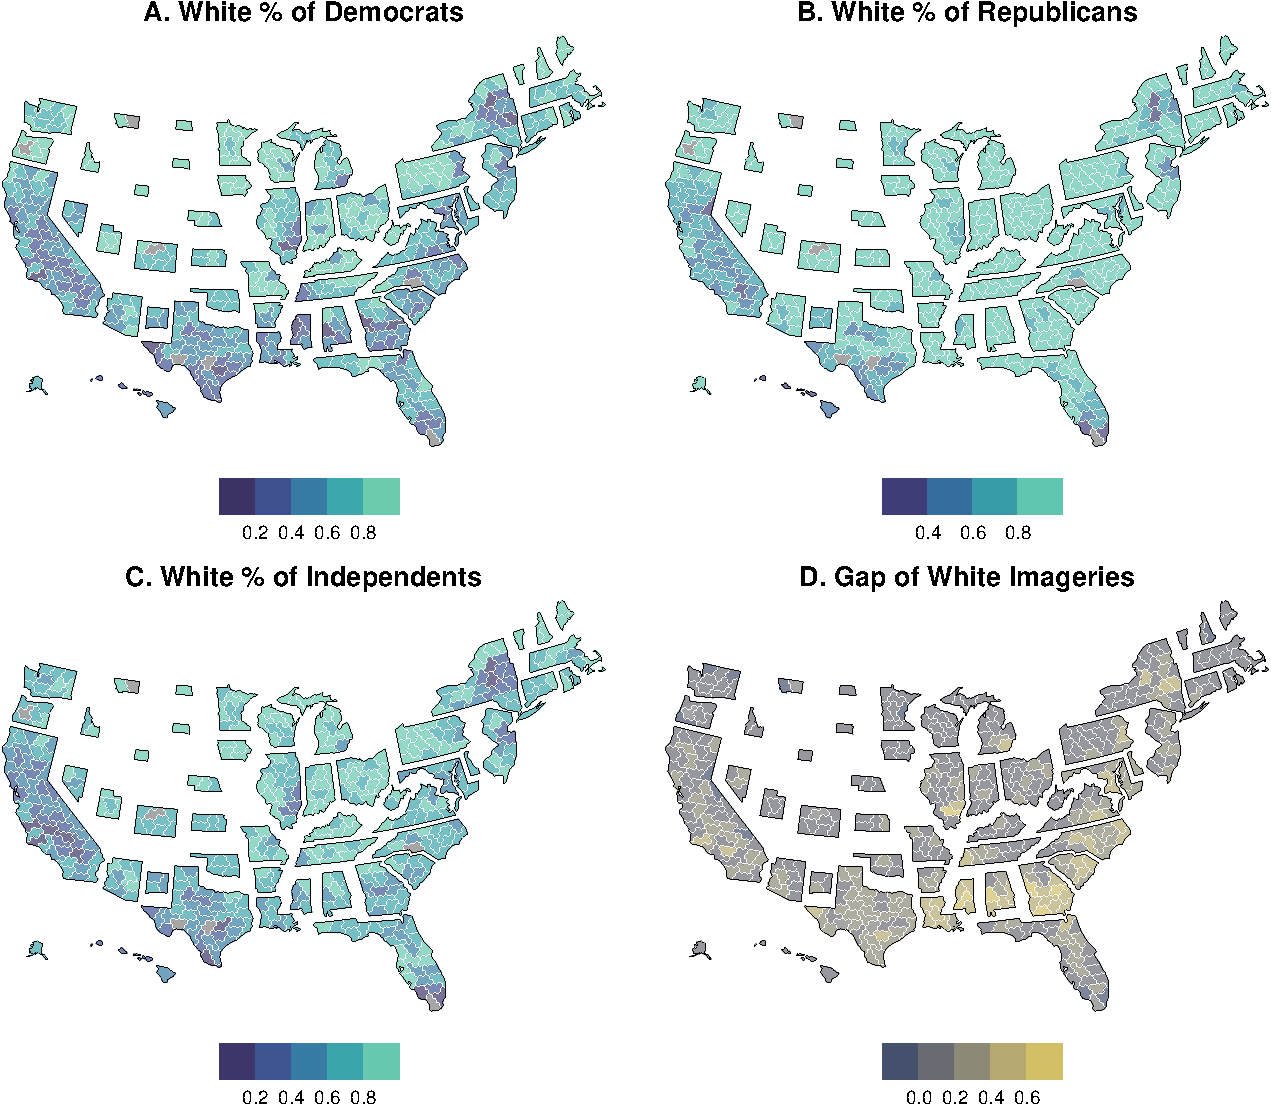
\includegraphics{local-images_files/figure-pdf/fig-map-1.pdf}

}

\caption{\label{fig-map}\textbf{Geograhpic Variation of Party Imageries
at the Level of Congressional Districts.} States are resized to be in
proportion to their population sizes, and districts are located within
the states to approximately match their actual locations. This cartogram
is created by the Daily Kos team (\url{https://www.dailykos.com}).}

\end{figure}

\begin{figure}[tb]

{\centering 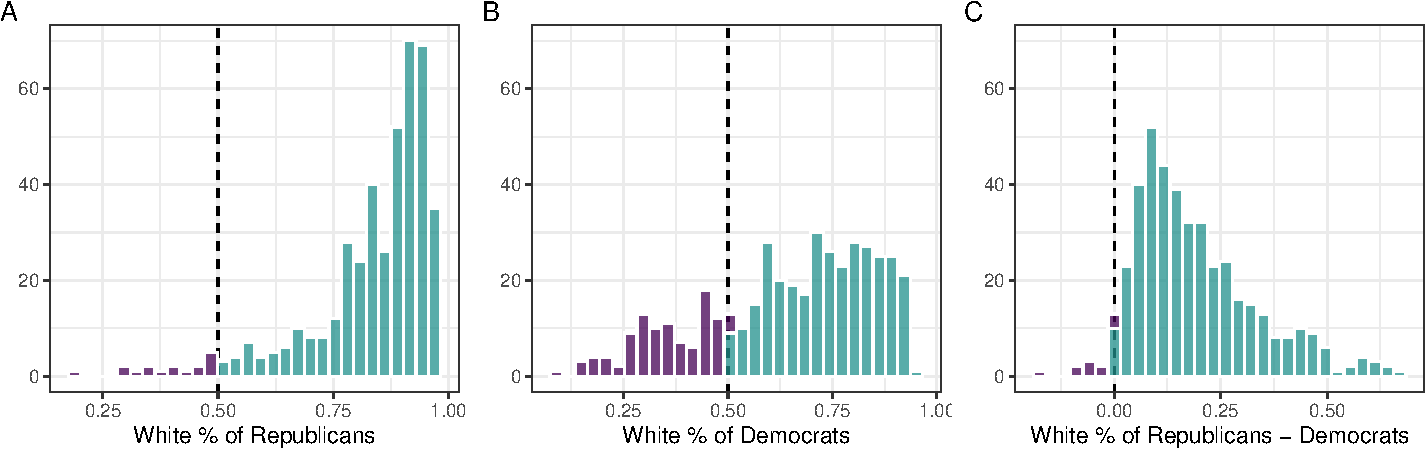
\includegraphics{local-images_files/figure-pdf/fig-hist-1.pdf}

}

\caption{\label{fig-hist}\textbf{Distribution of Party Imageries and
Their Gap among Congressional Districts.} The first two panels shows the
distribution of the percentages of non-Hispanic whites among the
Republican and Democratic partisans in a congressional district. The
last panel, capturing the contrast of the white imagery between
Republicans and Democrats, shows the distribution of the gap between the
two percentages.}

\end{figure}

\begin{figure}[tb]

{\centering 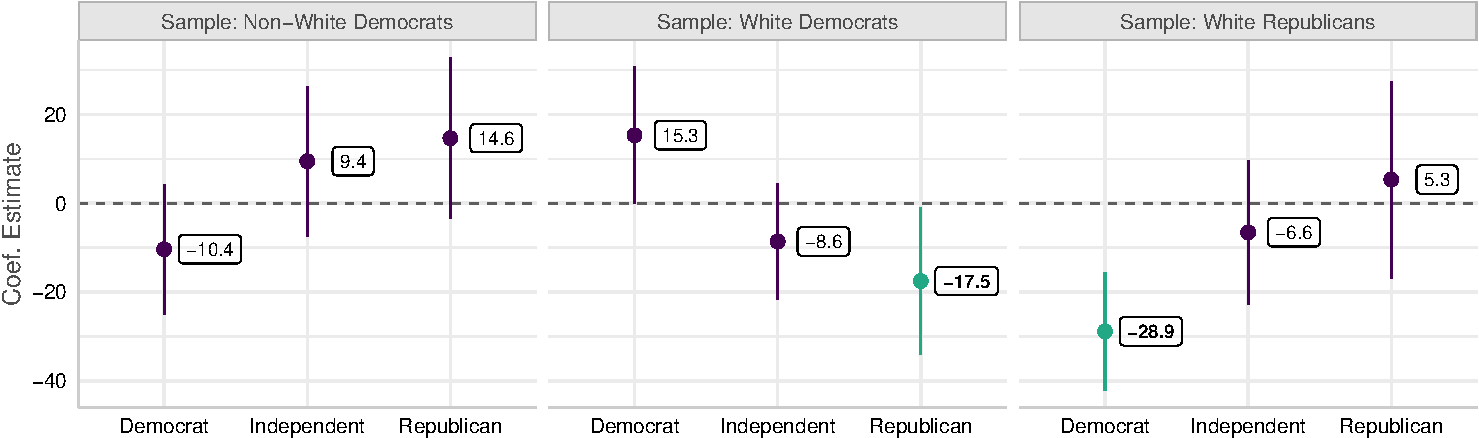
\includegraphics{local-images_files/figure-pdf/fig-baseline-1.pdf}

}

\caption{\label{fig-baseline}\textbf{The Estimated Effect of Party
Imageries on Affective Polarization by Different Types of Partisans.}
Panels indicates three subsamples of partisans in 2020 ANES. The labels
on the horizontal axis shows the party imagery of what political group
is of interest in a regression. A single point represents the estimated
effect of the district-level white imagery of a political group on the
affective polarization of the partisans in a congressional district, and
the range shows its 95\% confidence interval. Significant esimtates (p
\textless{} 0.05) are colored in green and marked in bold text. White
percentage of a district's population is controlled for.}

\end{figure}

\begin{figure}[tb]

{\centering 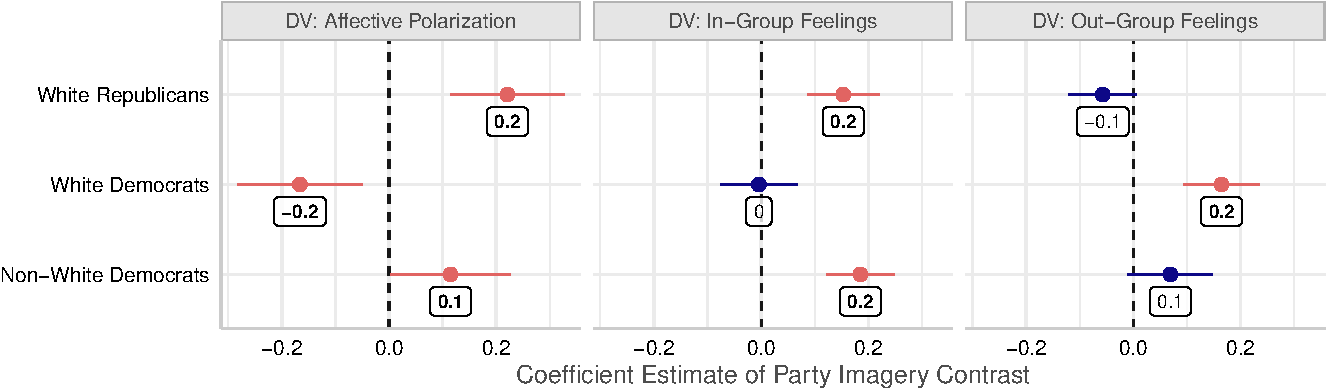
\includegraphics{local-images_files/figure-pdf/fig-decompose-1.pdf}

}

\caption{\label{fig-decompose}\textbf{The Estimated Effect of Party
Imagery on Affective Polarization, Broken Down by In-Group and Out-Group
Feelings.} Panels indicates three outcome variables pertaining to
affective polarization, and the labels on the vertical axis shows the
partisan subsample of 2020 ANES upon whom a regression is based. An
individual point represents the estimated effect that district-level
contrast of party imagery has on the outcome variable, and the range
shows its 95\% confidence interval. Significant esimtates (p \textless{}
0.05) are colored in red and marked in bold text. White percentage of a
district's population is controlled for.}

\end{figure}

\hypertarget{tbl-mechanism}{}
\begin{table}
\caption{\label{tbl-mechanism}Contrast of Party Images Moderates the Effect of White Feelings on
Affective Polarization }\tabularnewline

\centering
\begin{threeparttable}
\begin{tabular}[t]{lccc}
\toprule
  & Republican FT & Democrat FT & Rep. FT - Dem. FT\\
\midrule
White FT & 0.188*** & 0.016 & 0.168**\\
 & (0.029) & (0.030) & (0.053)\\
Party Imagery Contrast & 0.019 & 0.195* & -0.183\\
 & (0.081) & (0.093) & (0.150)\\
White FT × Party Imagery Contrast & 0.003** & -0.004** & 0.007***\\
 & (0.001) & (0.001) & (0.002)\\
\midrule
Observations & 6983 & 6989 & 6960\\
R squared & 0.053 & 0.033 & 0.046\\
\bottomrule
\end{tabular}
\begin{tablenotes}
\item Note: All respondents in 2020 ANES. FT means the respondent's feeling thermometer score of the group on a 100-point scale, higher values indicating more warmer feelings. The term Party Imagery Contrast refers to the contrast between Republicans and Democrats in terms of their white imagery. Robust standard errors in parentheses. + p $<$ 0.1, * p $<$ 0.05, ** p $<$ 0.01, *** p $<$ 0.001
\end{tablenotes}
\end{threeparttable}
\end{table}

\begin{figure}[tb]

{\centering 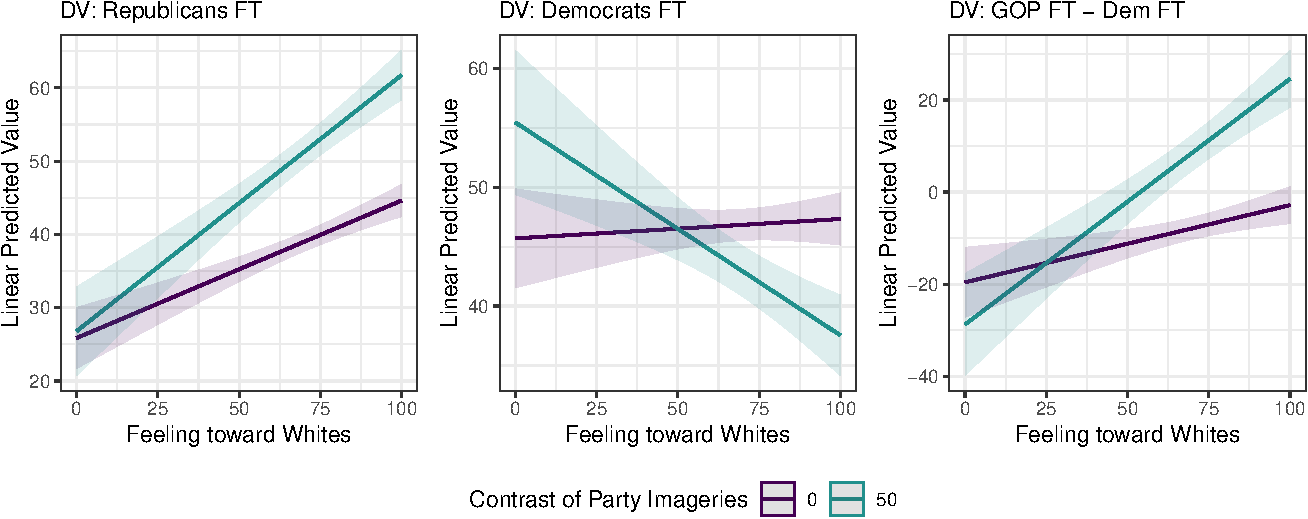
\includegraphics{local-images_files/figure-pdf/fig-mechanism-1.pdf}

}

\caption{\label{fig-mechanism}\textbf{Greater Contrast of Party Images
Accentuates the Influence of White Feelings on Voter's Affective
Perception of Political Parties.} Linear predicted values based upon the
previous OLS analyses with interaction terms between white FT and party
FT. Panels reponds to the three outcome variables. Within each panel,
the two ribbons plot how affective polarization changes as feelings
toward whites become warmer at two levels of party imagery contrast. The
bands show the 95\% confidcence internals.}

\end{figure}

\small

\hypertarget{references}{%
\section*{References}\label{references}}
\addcontentsline{toc}{section}{References}

\hypertarget{refs}{}
\begin{CSLReferences}{1}{0}
\leavevmode\vadjust pre{\hypertarget{ref-ahler2018}{}}%
Ahler, Douglas J., and Gaurav Sood. 2018. {``The Parties in Our Heads:
Misperceptions about Party Composition and Their Consequences.''}
\emph{The Journal of Politics} 80 (3): 964--81.
\url{https://doi.org/10.1086/697253}.

\leavevmode\vadjust pre{\hypertarget{ref-campbell2006}{}}%
Campbell, Andrea Louise, Cara Wong, and Jack Citrin. 2006. {``{``}Racial
Threat{''}, Partisan Climate, and Direct Democracy: Contextual Effects
in Three California Initiatives.''} \emph{Political Behavior} 28 (2):
129--50. \url{https://doi.org/10.1007/s11109-006-9005-6}.

\leavevmode\vadjust pre{\hypertarget{ref-carmines1990}{}}%
Carmines, Edward G., and James A. Stimson. 1990. \emph{Issue evolution:
race and the transformation of American politics}. Princeton, N.J.:
Princeton University Press.

\leavevmode\vadjust pre{\hypertarget{ref-downs1957}{}}%
Downs, Anthony. 1957. \emph{An Economic Theory of Democracy}. New York:
Harper Collins.

\leavevmode\vadjust pre{\hypertarget{ref-egan2020}{}}%
Egan, Patrick J. 2020. {``Identity as Dependent Variable: How Americans
Shift Their Identities to Align with Their Politics.''} \emph{American
Journal of Political Science} 64 (3): 699--716.
\url{https://doi.org/10.1111/ajps.12496}.

\leavevmode\vadjust pre{\hypertarget{ref-fiorina1981}{}}%
Fiorina, Morris P. 1981. \emph{Retrospective Voting in American National
Elections}. New Haven: Yale University Press.

\leavevmode\vadjust pre{\hypertarget{ref-green2002}{}}%
Green, Donald P., Bradley Palmquist, and Eric Schickler. 2002.
\emph{Partisan Hearts and Minds: Political Parties and the Social
Identities of Voters}. Yale ISPS Series. New Haven, CT; London: Yale
University Press.

\leavevmode\vadjust pre{\hypertarget{ref-hajnal2014}{}}%
Hajnal, Zoltan, and Michael U. Rivera. 2014. {``Immigration, Latinos,
and White Partisan Politics: The New Democratic Defection.''}
\emph{American Journal of Political Science} 58 (4): 773--89.
\url{https://doi.org/10.1111/ajps.12101}.

\leavevmode\vadjust pre{\hypertarget{ref-hopkins2009}{}}%
Hopkins, Daniel J. 2009. {``The Diversity Discount: When Increasing
Ethnic and Racial Diversity Prevents Tax Increases.''} \emph{The Journal
of Politics} 71 (1): 160--77.
\url{https://doi.org/10.1017/S0022381608090105}.

\leavevmode\vadjust pre{\hypertarget{ref-kane2021}{}}%
Kane, John V., Lilliana Mason, and Julie Wronski. 2021. {``Who{'}s at
the Party? Group Sentiments, Knowledge, and Partisan Identity.''}
\emph{The Journal of Politics} 83 (4): 1783--99.
\url{https://doi.org/10.1086/715072}.

\leavevmode\vadjust pre{\hypertarget{ref-mason2016}{}}%
Mason, Lilliana. 2016. {``A Cross-Cutting Calm: How Social Sorting
Drives Affective Polarization.''} \emph{Public Opinion Quarterly} 80
(S1): 351--77. \url{https://doi.org/10.1093/poq/nfw001}.

\leavevmode\vadjust pre{\hypertarget{ref-mason2018}{}}%
---------. 2018. \emph{Uncivil Agreement: How Politics Became Our
Identity}. Chicago, Illinois; London: The University of Chicago Press.

\leavevmode\vadjust pre{\hypertarget{ref-mason2018a}{}}%
Mason, Lilliana, and Julie Wronski. 2018. {``One Tribe to Bind Them All:
How Our Social Group Attachments Strengthen Partisanship.''}
\emph{Political Psychology} 39 (February): 257--77.
\url{https://doi.org/10.1111/pops.12485}.

\leavevmode\vadjust pre{\hypertarget{ref-newman2015}{}}%
Newman, Benjamin J., Yamil Velez, Todd K. Hartman, and Alexa Bankert.
2015. {``Are Citizens {``}Receiving the Treatment{''}? Assessing a Key
Link in Contextual Theories of Public Opinion and Political Behavior:
Receiving the Treatment.''} \emph{Political Psychology} 36 (1): 123--31.
\url{https://doi.org/10.1111/pops.12069}.

\leavevmode\vadjust pre{\hypertarget{ref-valentino2005}{}}%
Valentino, Nicholas A., and David O. Sears. 2005. {``Old Times There Are
Not Forgotten: Race and Partisan Realignment in the Contemporary
South.''} \emph{American Journal of Political Science} 49 (3): 672--88.
\url{https://doi.org/10.1111/j.1540-5907.2005.00136.x}.

\leavevmode\vadjust pre{\hypertarget{ref-westwood2020}{}}%
Westwood, Sean J., and Erik Peterson. 2020. {``The Inseparability of
Race and Partisanship in the United States.''} \emph{Political
Behavior}, October. \url{https://doi.org/10.1007/s11109-020-09648-9}.

\leavevmode\vadjust pre{\hypertarget{ref-wong2010}{}}%
Wong, Cara. 2010. \emph{Boundaries of Obligation in American Politics:
Geographic, National, and Racial Communities}. Cambridge Studies in
Public Opinion and Political Psychology. Cambridge {[}England{]} ; New
York: Cambridge University Press.

\leavevmode\vadjust pre{\hypertarget{ref-zhirkov2022}{}}%
Zhirkov, Kirill, and Nicholas A. Valentino. 2022. {``The Origins and
Consequences of Racialized Schemas about U.S. Parties.''} \emph{The
Journal of Race, Ethnicity, and Politics}, April, 1--21.
\url{https://doi.org/10.1017/rep.2022.4}.

\end{CSLReferences}



\end{document}
